\documentclass{article}
\usepackage{colm2026_conference}
\usepackage{times}
\usepackage{url}
\usepackage{graphicx}
\usepackage{booktabs}
\usepackage{amsmath}

\title{Structural Geometry, Not Sparsity, Breaks Reasoning Under LLM Compression}

\author{Anonymous Authors \\
Paper under double-blind review
}

%\colmfinalcopy

\begin{document}
\maketitle

\begin{abstract}
Compression methods for large language models are often validated with general language-modeling perplexity, but reasoning workloads can fail even when perplexity degradation appears modest. We study this mismatch on Mistral-7B using GSM8K as a reasoning benchmark and C4 perplexity as a general language-modeling control. Hardware-aligned structural MLP-width pruning sharply degrades GSM8K even at low sparsity, while dense-shaped layerwise magnitude masks preserve most reasoning accuracy at substantially higher sparsity. A 20\% dense-shaped mask reaches 37.23\% GSM8K strict exact match on the full 1,319-example test set, compared with 38.67\% for the dense baseline, a gap of only 1.44 points. Its generated solutions also preserve chain length: 57.05 average response words versus 56.58 for dense. By contrast, structural 20\% width pruning collapses full GSM8K to roughly 5\% despite remaining a recognizable language model under C4 perplexity. These results show that reasoning retention is governed by structural geometry, not sparsity alone, and motivate compression methods that preserve reasoning-critical subspace geometry before targeting hardware speedups.
\end{abstract}

\section{Introduction}

Efficient reasoning requires more than reducing parameter count or preserving average next-token loss. Compression can keep a model fluent while damaging the internal geometry needed for multi-step reasoning. This creates a practical failure mode for deployment: a compressed model can look acceptable on C4 perplexity while failing GSM8K.

This paper isolates that failure mode with a paired control. We compare two ways of removing capacity from Mistral-7B:
\begin{enumerate}
    \item \textbf{Structural MLP-width pruning}: physically narrows feed-forward dimensions, creating real shape changes and potential hardware speedups.
    \item \textbf{Dense-shaped magnitude masking}: zeros weights layerwise while preserving the original dense parameter geometry and tensor shapes.
\end{enumerate}

The control is intentionally asymmetric from a systems perspective. Dense-shaped masks do not produce structural speedups. Their role is diagnostic: if a dense-shaped 20--30\% mask preserves GSM8K while much smaller structural width changes collapse it, then reasoning loss cannot be attributed to sparsity or C4 degradation alone.

\section{Experimental Setup}

We evaluate Mistral-7B-v0.1 under 5-shot GSM8K with deterministic generation. C4 validation perplexity is computed as a general language-modeling control. Structural pruning uses hardware-aligned MLP-width pruning; mask pruning applies layerwise unstructured magnitude masks to all linear layers while preserving the original dense tensor shapes.

All checkpoints and evaluation scripts are implemented in the repository. The live Phase 19 summary table is generated with:

\begin{verbatim}
python scripts/summarize_phase19.py
\end{verbatim}

The GSM8K generation-length sanity check is generated with:

\begin{verbatim}
python scripts/analyze_phase19_samples.py
\end{verbatim}

\section{Results}

\subsection{Dense-Shaped Masks Preserve Reasoning at 20\% Sparsity}

Table~\ref{tab:phase19_mask} shows the current Phase 19 mask-control results. The 20\% mask result is complete on the full GSM8K test set. The 30\% and 40\% rows currently show 50-example smoke metrics while full evaluations are running.

\begin{table}[h]
\centering
\caption{Phase 19 dense-shaped mask controls on Mistral-7B. Full GSM8K uses 1,319 examples; smoke rows use 50 examples and are marked accordingly.}
\label{tab:phase19_mask}
\begin{tabular}{lrrrrr}
\toprule
\textbf{Model/state} & \textbf{Sparsity} & \textbf{C4 PPL} & \textbf{GSM8K n} & \textbf{Strict EM} & \textbf{$\Delta$ vs dense} \\
\midrule
Dense Mistral-7B & 0.0\% & 8.013 & 1319 & 38.67\% & 0.00 \\
Mask pruning & 20.0\% & 8.195 & 1319 & 37.23\% & -1.44 \\
Mask pruning & 30.0\% & 8.586 & 50 & 36.00\% & smoke \\
Mask pruning & 40.0\% & 9.538 & 50 & 28.00\% & smoke \\
\bottomrule
\end{tabular}
\end{table}

The 20\% mask is the key positive control: it removes roughly one fifth of linear weights while retaining GSM8K within 1.44 points of the dense baseline. This establishes that substantial weight-level sparsity is not sufficient to explain reasoning collapse. The result is not explained by terse or malformed generations: the full-run sample log shows 57.05 average generated words for the 20\% mask versus 56.58 for the dense baseline, with final-answer-marker rates of 88.7\% and 90.5\%, respectively.

\subsection{Structural Width Pruning Fails Much Earlier}

The paired structural runs show the opposite behavior. Phase 18B structural width pruning smoke tests degrade GSM8K sharply even at 1--5\% sparsity, and Phase 16 full structural 20\% width pruning drops GSM8K to roughly 5\%. This contrast is the central dissociation:

\begin{itemize}
    \item Dense-shaped 20\% mask: near-dense full GSM8K.
    \item Structural 1--5\% width pruning: sharp GSM8K smoke degradation.
    \item Structural 20\% width pruning: full GSM8K collapse.
\end{itemize}

\begin{figure}[h]
\centering
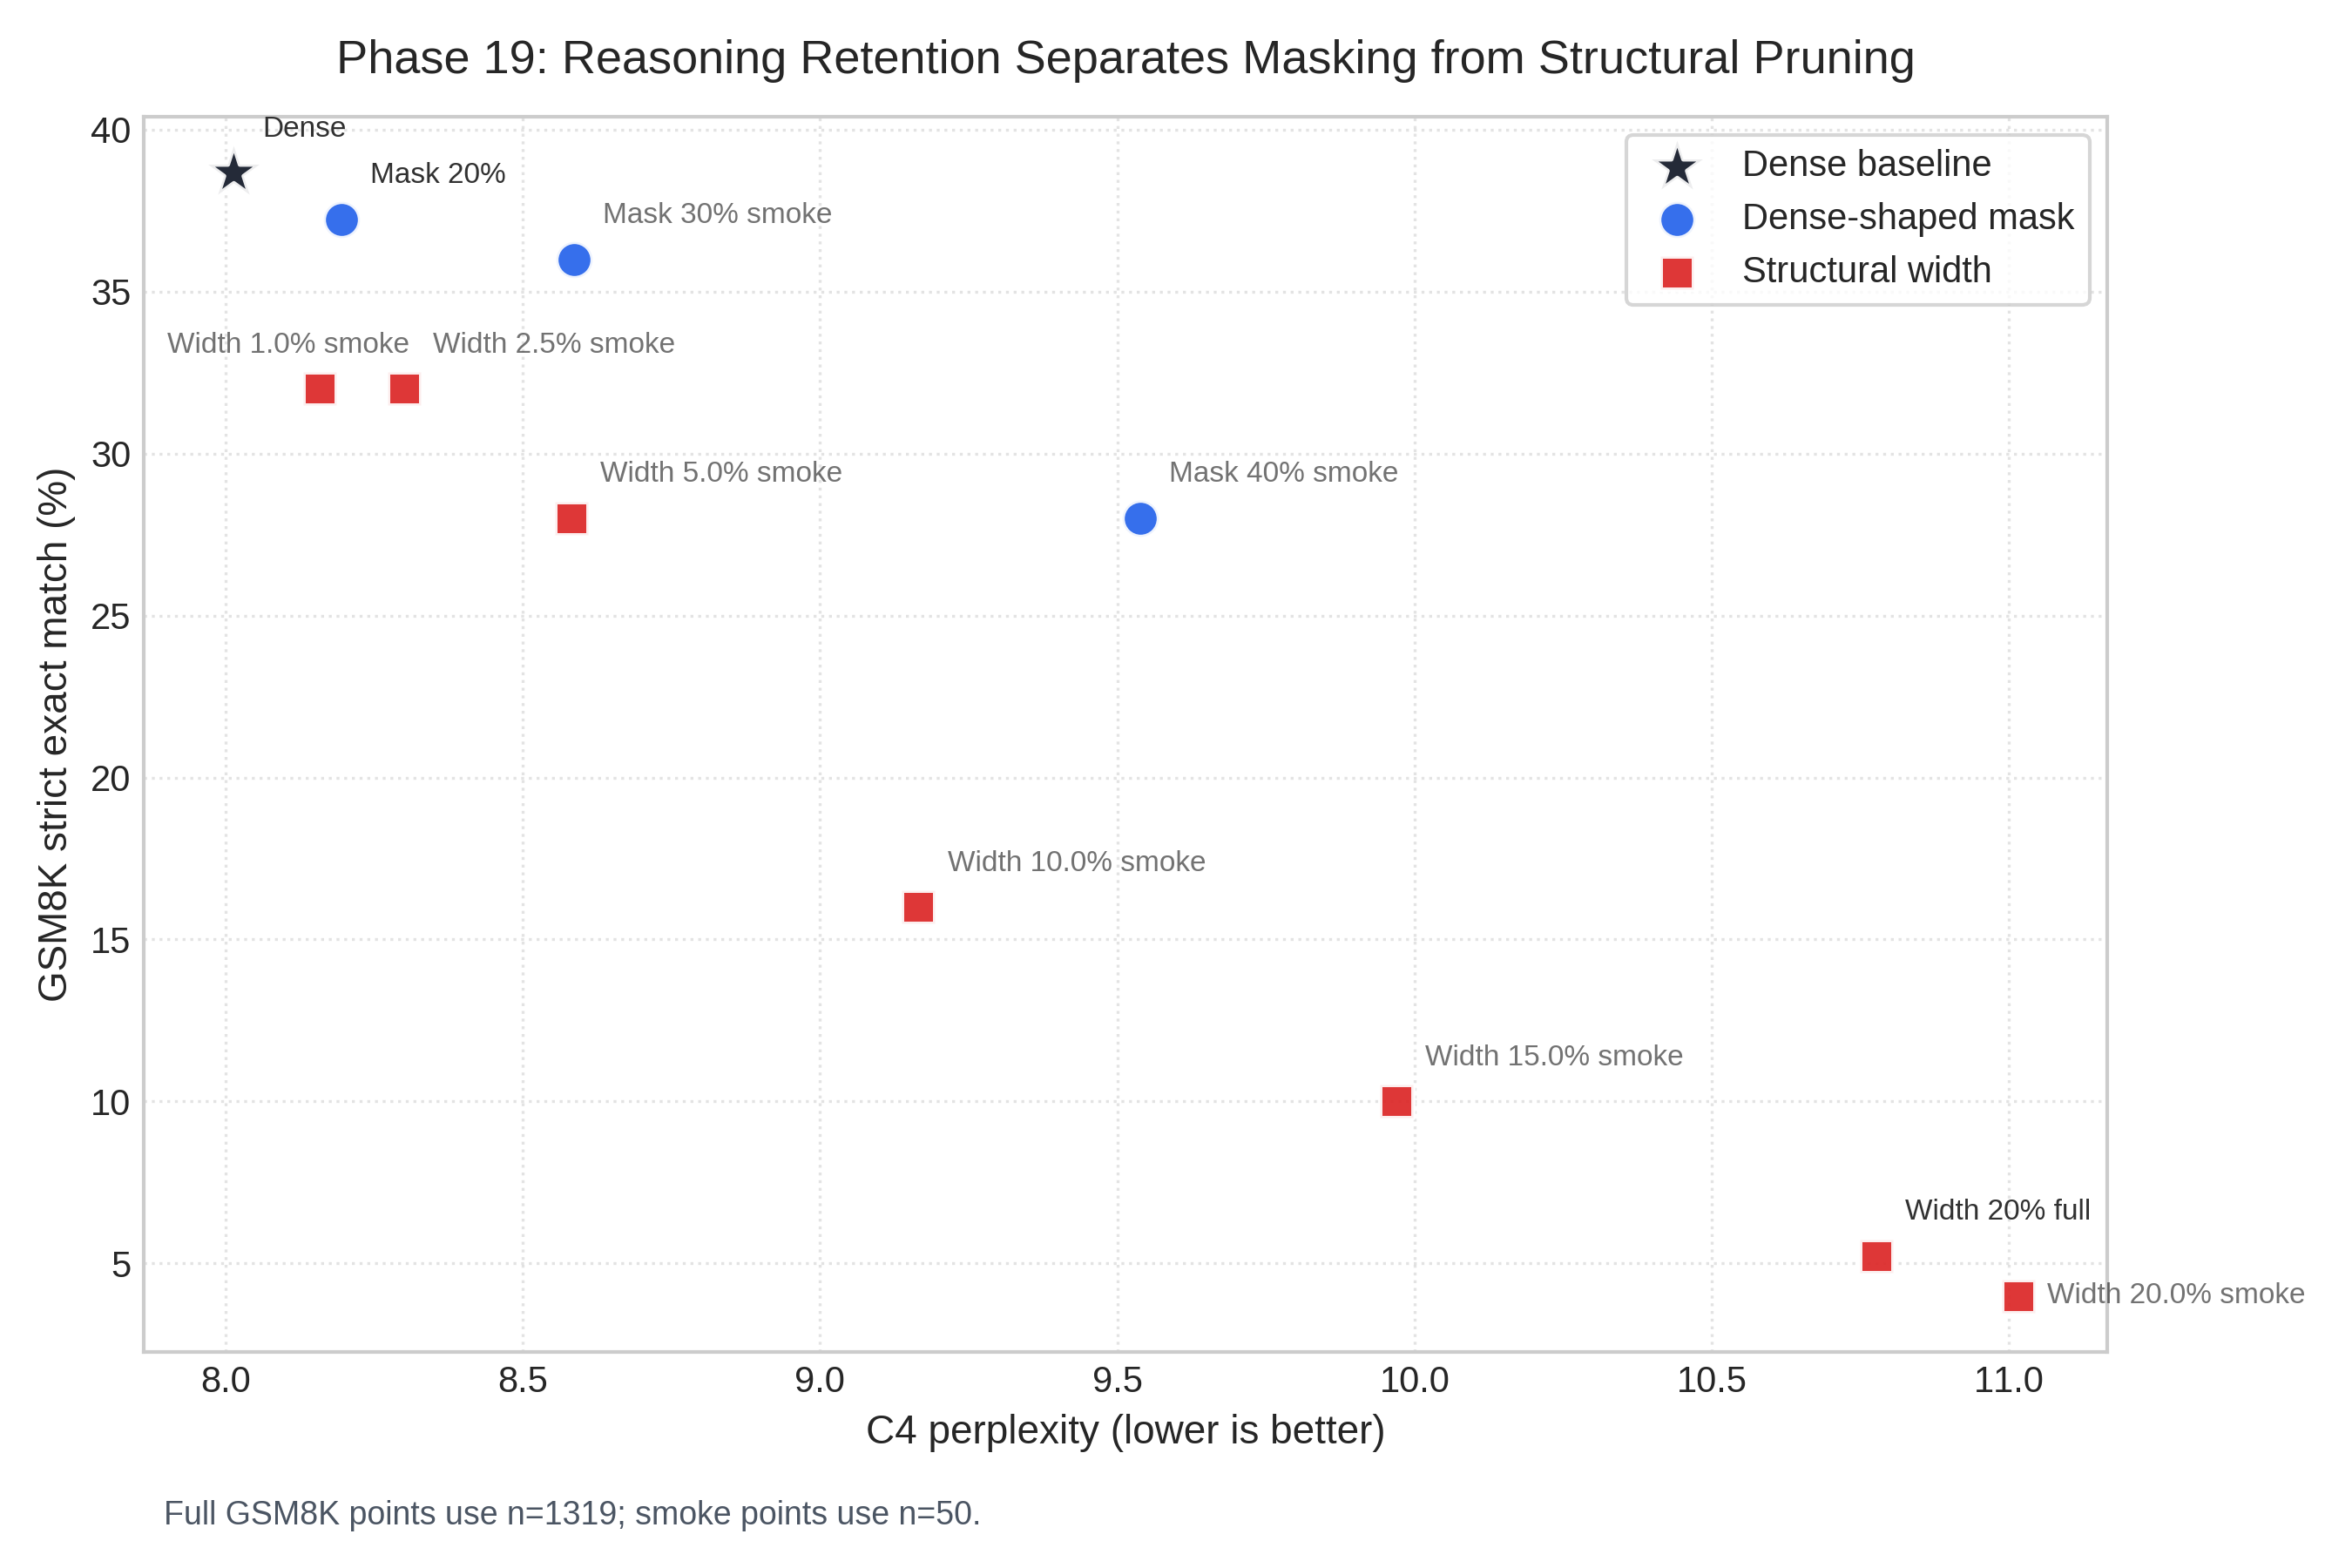
\includegraphics[width=\textwidth]{figures/phase19_reasoning_dissociation.png}
\caption{C4 perplexity versus GSM8K strict exact match for dense, dense-shaped mask, and structural width pruning controls. The current full 20\% mask point remains near dense, while structural width points fall away rapidly. Full 30\% and 40\% mask evaluations are running and will replace the smoke annotations once complete.}
\label{fig:phase19_dissociation}
\end{figure}

\section{Interpretation}

The result suggests that reasoning degradation is not controlled by sparsity alone. Dense-shaped masks perturb weights but preserve the model's original layer dimensions, residual interfaces, and tensor geometry. Structural width pruning changes those interfaces and can disrupt reasoning-critical subspaces even when C4 perplexity remains in a plausible range.

This has two implications for efficient reasoning:
\begin{enumerate}
    \item Perplexity-only validation is insufficient for reasoning compression.
    \item Hardware speedups should be pursued only after identifying structural transformations that preserve the reasoning-retained subspace exposed by the mask control.
\end{enumerate}

\section{Next Evidence}

Two full GSM8K evaluations are currently running for 30\% and 40\% dense-shaped masks. If the 30\% mask remains near dense, the paper can claim a broad mask-retention regime. If 30\% degrades but 20\% remains near dense, the paper still establishes a thresholded dissociation: structural pruning fails substantially earlier than dense-shaped masking. An adaptive boundary run is queued to evaluate either 35\% or 25\% next, depending on the completed 30\% result.

\section{Conclusion}

Phase 19 reframes the compression problem for reasoning models. The immediate bottleneck is not whether parameters can be removed, but whether the structural geometry that carries reasoning behavior survives the compression operator. Dense-shaped masks provide a strong positive control, while hardware-aligned structural width pruning provides a strong negative control. Together they motivate a new target for efficient reasoning compression: preserve reasoning-critical geometry first, then recover hardware efficiency.

\bibliography{colm2026_conference}
\bibliographystyle{colm2026_conference}

\end{document}
